\chapter{Diagrama de Casos de Uso} \label{cha:diagramacasouso}

Neste capítulo é apresentado o diagrama de casos de uso do aplicativo proposto, onde é possível visualizar de forma clara e organizada as principais funcionalidades e interações entre os atores (Usuário e Lojista) e o sistema. O diagrama de casos de uso oferece uma visão geral das ações que podem ser realizadas pelos usuários do aplicativo, como buscar produtos, comparar preços, cadastrar produtos, entre outras.

%DUVIDA: cada caso de uso = tela = historia?

\imagem{DIAGRAMA DE CASOS DE USO}{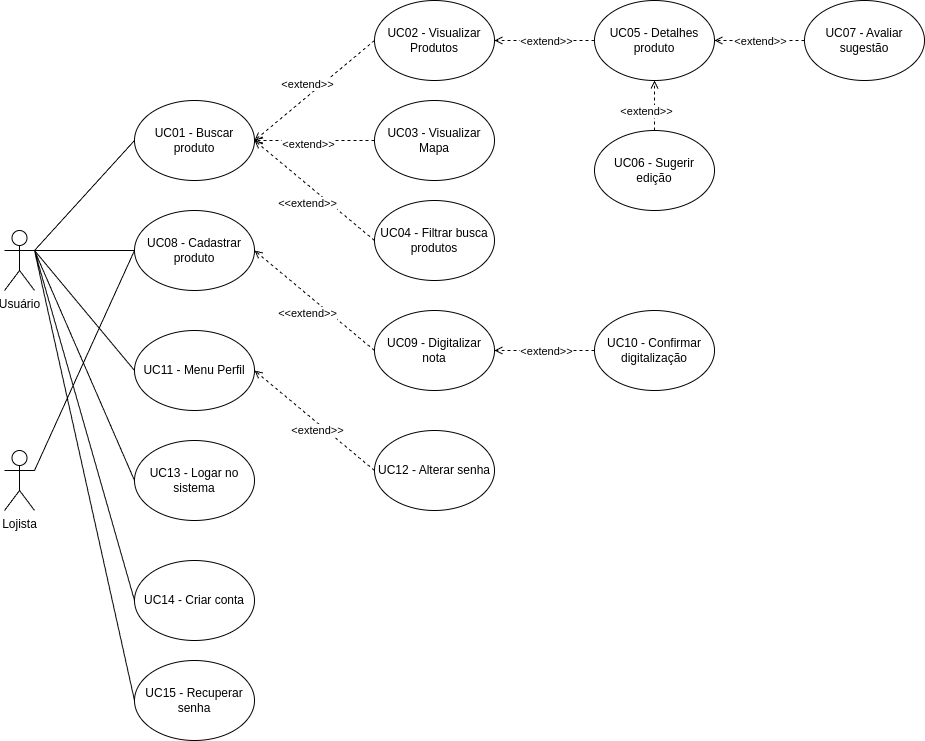
\includegraphics[width = 170mm]{fig/usecase.drawio.png}}{O Autor (2024)}{usecase}{nota(s)}{legenda(s)}